\newpage
\section{Begriffserklärung}
\label{Begriffe}
Ein Sudoku besteht aus 81 \textit{Feldern} oder \textit{Zellen}. In diese werden die \textit{Ziffern} oder \textit{Zahlen} eingetragen und sie bilden ein Quadrat der Größe 9x9, das \textit{Grid}. Aufgrund dieser Aufteilung hat ein Sudoku 9 \textit{Zeilen} und 9 \textit{Spalten}. Das Grid wird in 9 Unterquadrate geteilt, die jeweils 3x3 Felder groß sind. Diese werden \textit{Blöcke} genannt. Zeilen, Spalten und Blöcke werden unter dem Begriff \textit{Figur} zusammengfasst. Die Nummerierung der Blöcke erfolgt zeilenweise von links oben nach rechts unten.\\

\begin{figure}[h]
\begin{center}
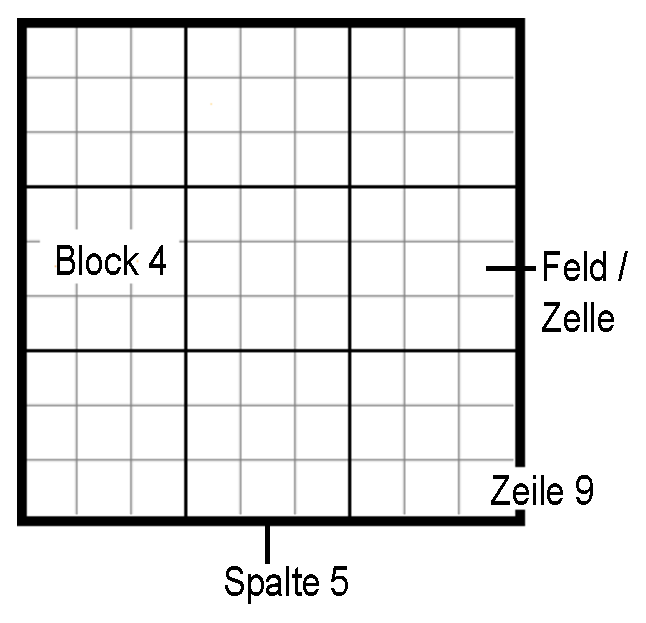
\includegraphics{./img/begriffe.eps}
\caption{Sudoku}
\end{center}
\end{figure}

\noindent In \textbf{Abbildung 2.2} sind diese Begriffe beispielhaft auf einem Spielfeld markiert.